\subsection{Ether}
Ether~\cite{ether} is a malware analysis platform that utilizes Intel VT's hardware virtualization extensions, and theoretically it has no presence in the guest operating system. It uses native CPU instructions, thus does not suffer from incomplete or inaccurate system emulation such as hardware emulators do. Ether also comes with a rich feature set, thus it can monitor all the memory write attempts of the guest, trace the instructions and system calls of in-guest processes, and unpack a wide range of protected binaries. As a result, malware cannot detect the presence of Ether. In that paper, they evaluated Ether and several other state-of-the-art analyzers on the obfuscation techniques used to obfuscate 25,000 recent malware samples. The results show that Ether remains transparent and defeats the obfuscation tools that evade the existing approaches. Ether's system architecture is represented in Figure~\ref{fig:ether} below.

\begin{figure}[!h]
	\centering
	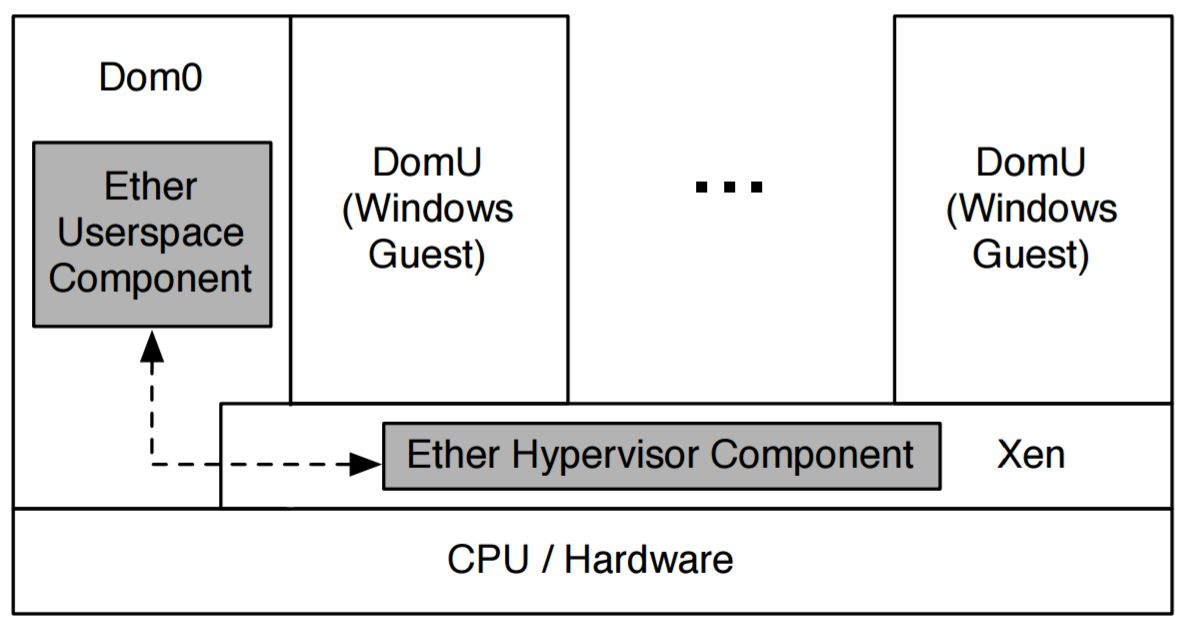
\includegraphics[width=\linewidth]{figure/ether.png}
	\caption{Ether's system architecture.}
	\label{fig:ether}
\end{figure}

\subsection{nEther}
nEther~\cite{nether} introduced new detection attacks against the out-of-the-guest malware analysis framework \textit{Ether}~\cite{ether}.

\begin{figure}[!h]
	\centering
	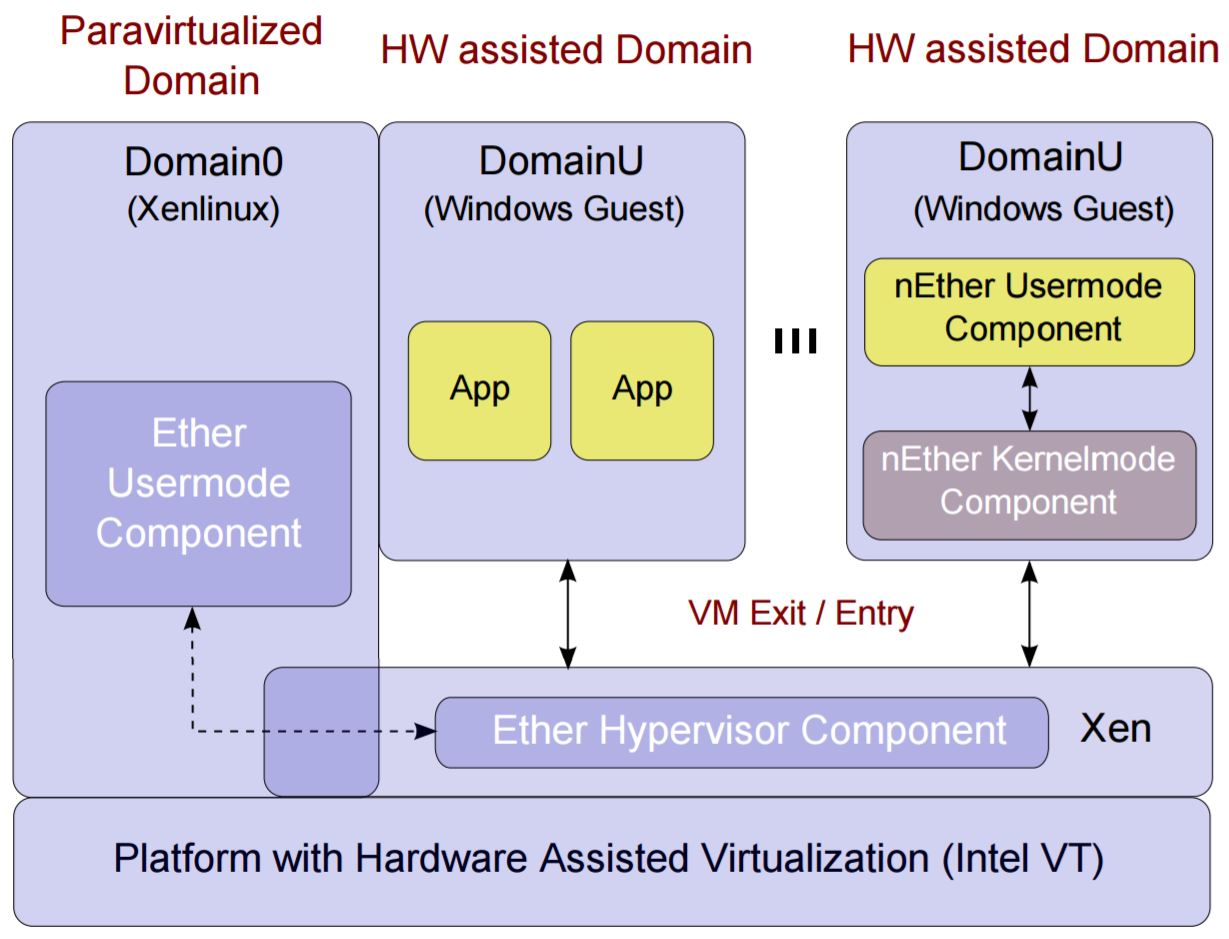
\includegraphics[width=\linewidth]{figure/nether.png}
	\caption{nEther's system overview.}
	\label{fig:nether}
\end{figure}

\subsection{title}

\mvf{TODO: CPU Errata~\cite{thompson}}

Several efforts has been made on how relative difference in execution time of
two instructions could be used to detect a virtualized
environment~\cite{raffetseder2007, thompson}. Using absolute time differences is
not feasible, as architectures are complex and different, but the relative
difference is more predictable. Comparing one instruction that is known not to
be trapped by the VMM and one that is, for instance {\tt NOP} and {\tt CPUID}
the authors showed that different VMMs showed significantly different ratios
compared to bare metal.

Ferrie {et al.} showed in 2007 how~\cite{ferrie2007} context switches between an
VMM and guest could be used to detect hypervisors based on Intel VT-x though the
flushing of the Translation Lookaside Buffer (TLB). Using a non-privileged
instruction that is still trapped by the VMM, i.e. {\tt CPUID}, will cause a
flush of the TLB. This could be detected through timing the instruction before
and after anticipated flush. This method has later been documented by other
authors~\cite{thompson}.
\mvf{Maybe not relevant with use of ASID? (doesn't flush TLB)}

Using dynamic analysis to disable detection routines~\cite{kang2009}.

Using remote detector machine~\cite{franklin2008}.

%%% Local Variables:
%%% mode: latex
%%% TeX-master: "../paper"
%%% End:
